\chapter{Further Plots}

\begin{figure}[h]
	\begin{center}
	  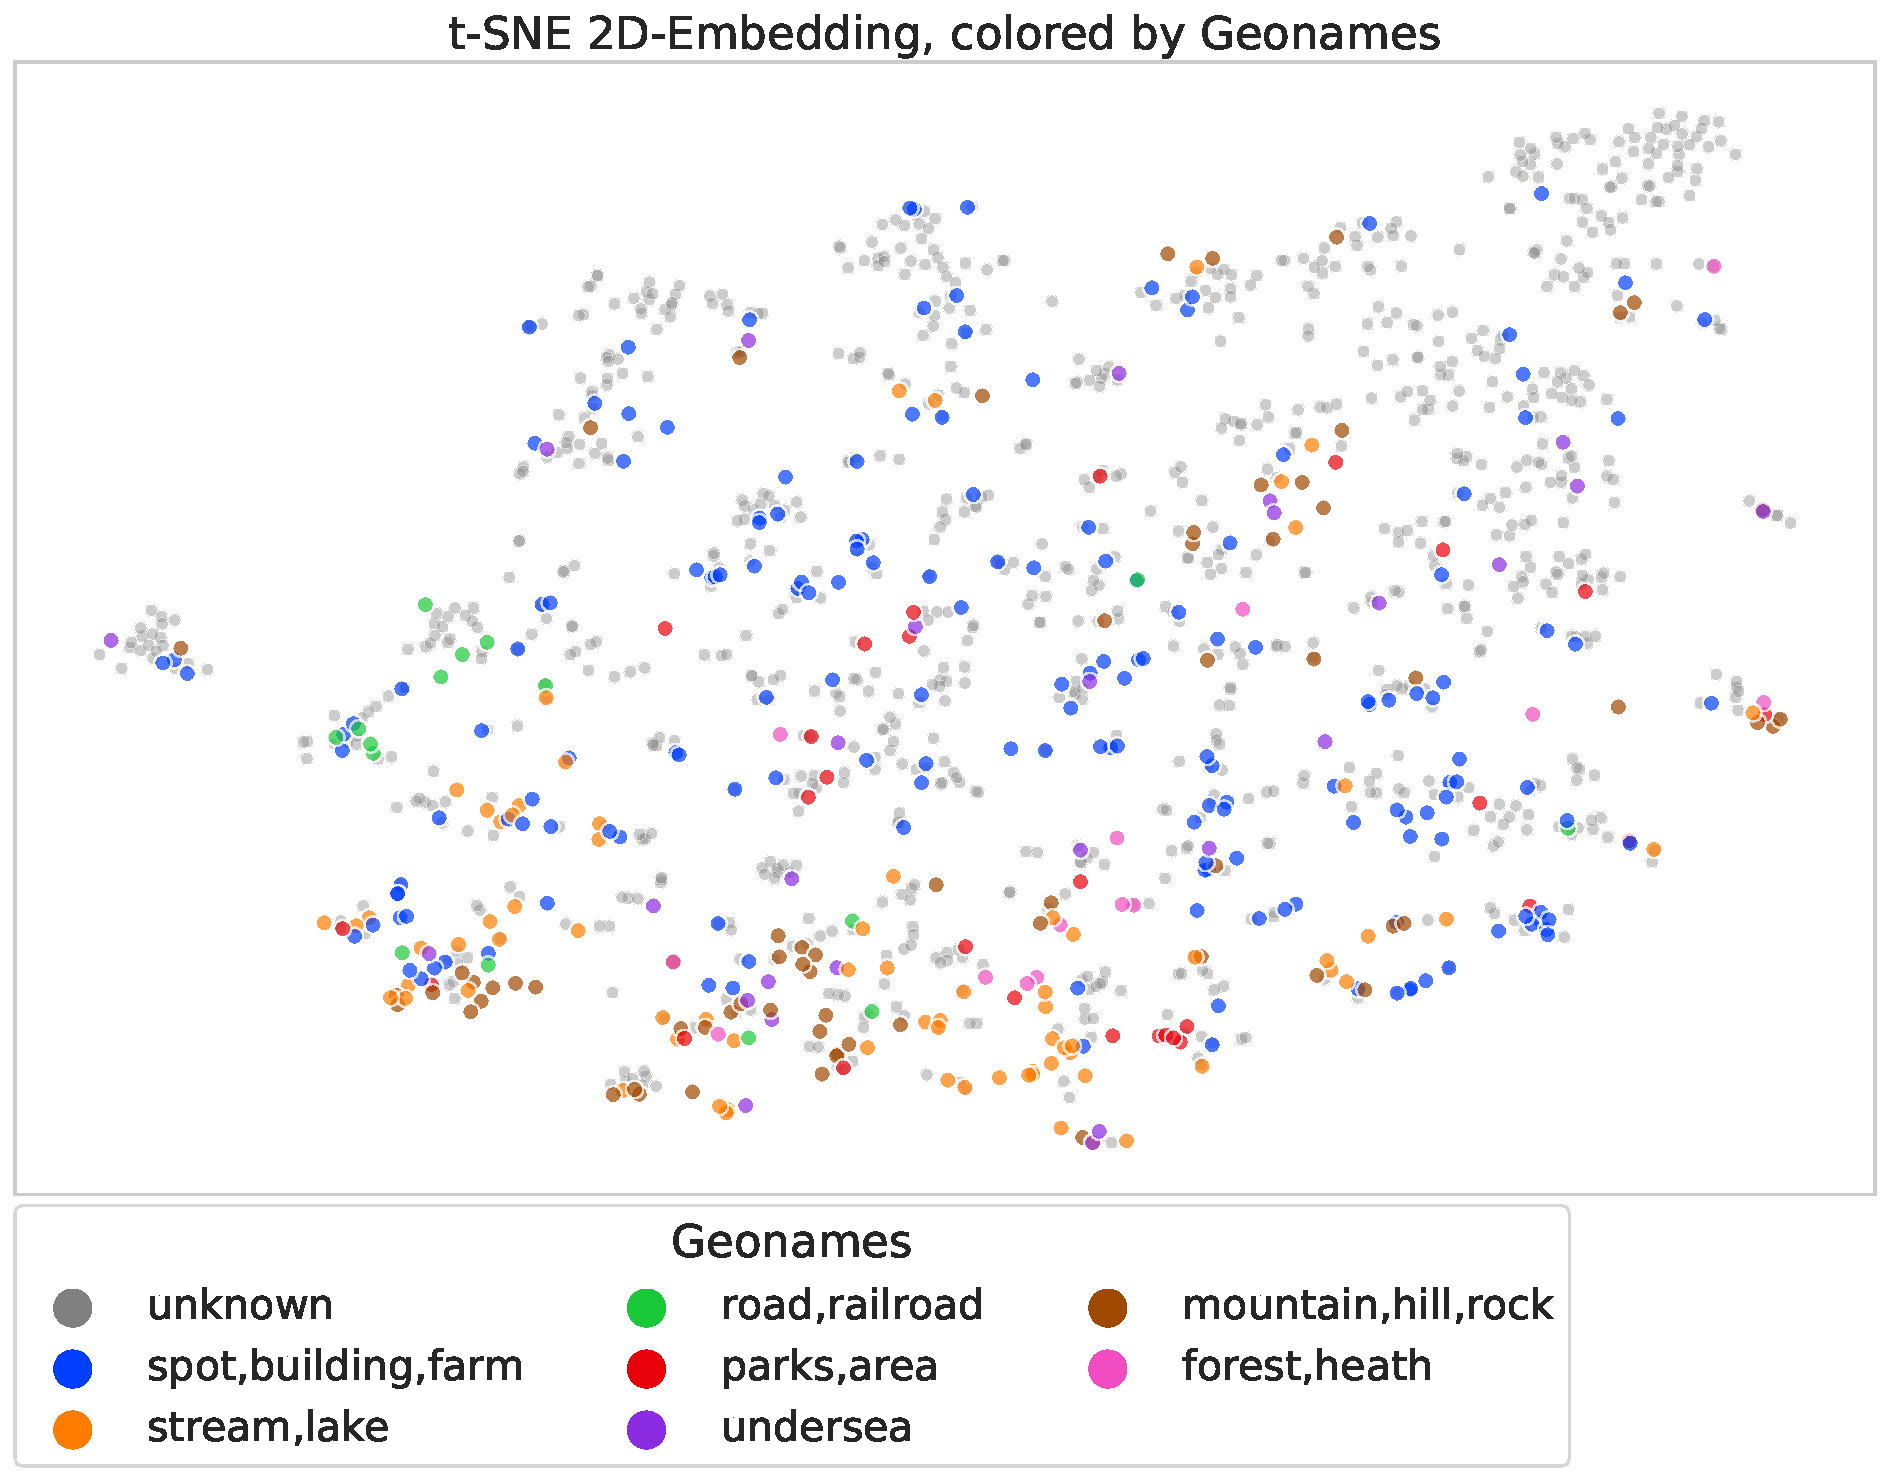
\includegraphics[width=\textwidth]{graphics/figures/scatter_mds_tsne_places_Geonames.pdf}
	  \slcaption{2D Visualization of the Placetypes-Dissimilarity-Matrix, generated with \gls{tsne}. See \url{https://github.com/cstenkamp/derive_conceptualspaces/blob/main/notebooks/text_referenced_plots/desc15_mds_2d3d.ipynb} for the origin of this plot.}
	  \label{fig:scatter_mds_placetypes}
      %TODO: "colored by Geonames"
	\end{center}
\end{figure}


\begin{figure}[h]
	\begin{center}
	  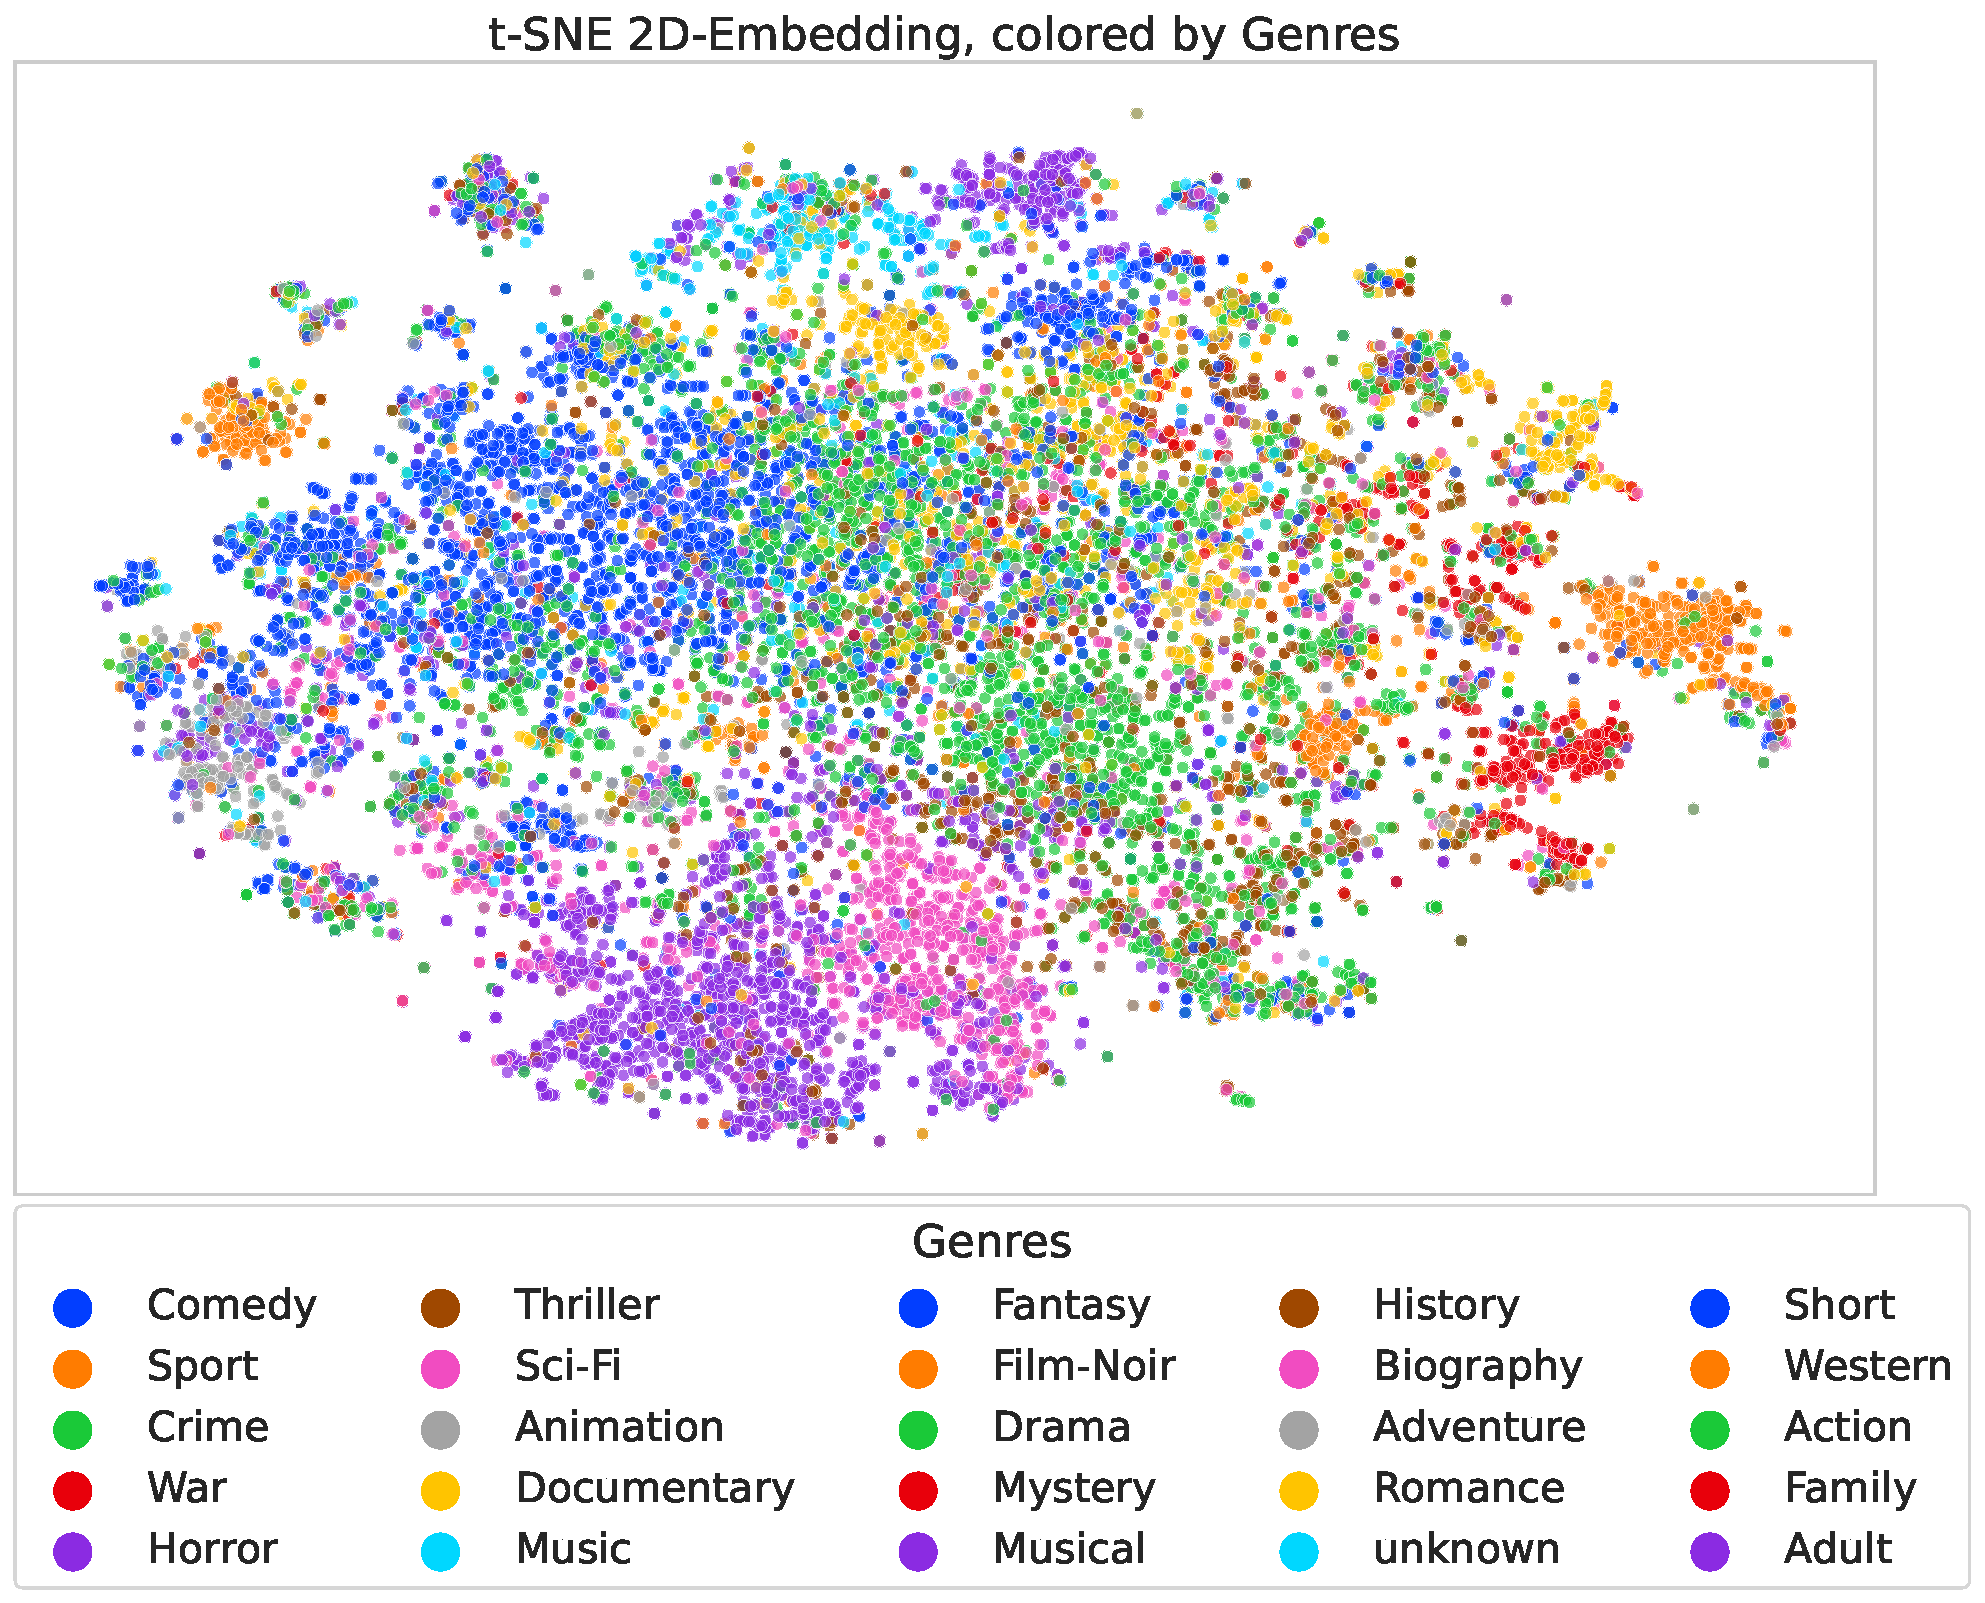
\includegraphics[width=\textwidth]{graphics/figures/scatter_mds_tsne_movies_Genres.pdf}
	  \slcaption{2D Visualization of the Movie-Dissimilarity-Matrix, generated with \gls{tsne}. See \url{https://github.com/cstenkamp/derive_conceptualspaces/blob/main/notebooks/text_referenced_plots/desc15_mds_2d3d.ipynb} for the origin of this plot.}
	  \label{fig:scatter_mds_movies}
      %TODO: "colored by genre"
	\end{center}
\end{figure}


\todoparagraph{Note that at} \url{https://github.com/cstenkamp/derive_conceptualspaces/blob/main/notebooks/text_referenced_plots/desc15_mds_2d3d.ipynb} there are also interactive 3D-Versions of these plots. The one for the SIDDATA-dataset is at \url{https://github.com/cstenkamp/derive_conceptualspaces/blob/main/notebooks/text_referenced_plots/visualize_embeddings.ipynb}, also 2D and interactive 3D. 